\documentclass[a4paper,add-index]{cnltx-doc}

\usepackage{syntaxdi}

\usepackage{hyperref}

\setcnltx{
    name     = syntaxdi ,
    title    = syntaxdi ,
    version  = 0.8.2 ,
    date     = 2020-10-16 ,
    subtitle = {\LaTeX-Paket zum Setzen von Syntaxdiagrammen in Form von Railroaddiagrammen},
    info     = Paketdokumentation ,
    authors  =  {Johannes Pieper, Johannes Kuhaupt, Ludger Humbert, Andr\'e Hilbig, Adrian Salamon, Daniel Spittank} ,
    email    = schulepaket@johpie.de ,
    url     = https://ddi.uni-wuppertal.de/material/schulepaket.html ,
    abstract = {%
        Mit diesem Paket werden Styles für TikZ bereit gestellt, um spezielle Syntaxdiagramme erstellen zu können. Diese sind auch als Railroaddiagramme bekannt und wurden von Niklaus Wirth zur Dokumentation der Syntax von Pascal eingeführt. In der Dokumentation des Pakets \pkg{pgf} wird die Erstellung in dem Tutorium \textbf{Diagrams as Simple Graphs} (S.~66--74) Schritt für Schritt beschrieben. Das Paket war vormals Teil des Schulepakets.
    } ,
    index-setup = { othercode=\footnotesize,level=\section},
    add-listings-options= {
        morekeywords={
        }
    },
}

\begin{document}

\section{Syntaxdiagramme}
\label{paket:syntaxdi}

Mit den Paketen \pkg{syntaxdi} und \pkg{tikz} ist es möglich, spezielle Syntaxdiagramme als Railroaddiagramme zu erstellen. Dazu sind Elemente definiert worden, die automatisch durch Pfeile miteinander verbunden werden.

Hierzu definiert das Paket \pkg{syntaxdi} einige TikZ-Stile, die einfach genutzt werden können.

\subsection{TikZ-Stile}
\begin{options}
    \opt{nonterminal} definiert ein Non-Terminal.
	\opt{terminal} definiert ein Terminal.
    \opt{fnonterminal} definiert ein Non-Terminal ohne automatische Verzweigung.
    \opt{fterminal} definiert ein Terminal ohne automatische Verzweigung.
    \opt{point} definiert einen Punkt, der ohne ankommenden Pfeil gezeichnet wird.
    \opt{endpoint} definiert einen Punkt, der mit ankommenden Pfeil gezeichnet wird.
\end{options}

\subsection{Beispiel}

Damit kann z.\,B. das Syntaxdiagramm für eine Mehrfachverzweigung in der Programmiersprache Python in Form eines Railroaddiagramms dargestellt werden.

\begin{example}[gobble=0]
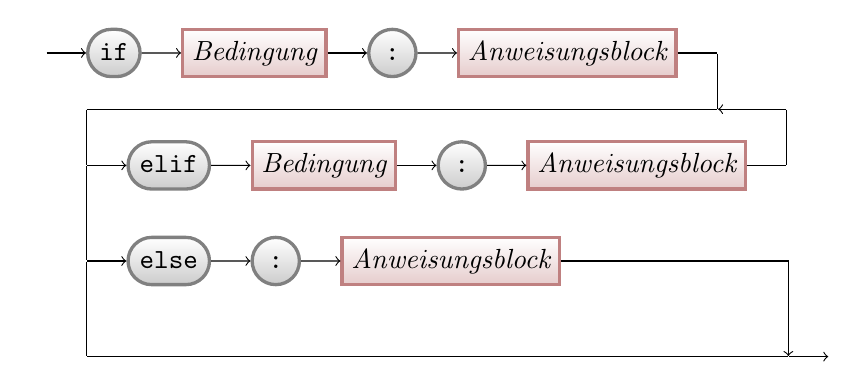
\begin{tikzpicture}[syntaxdiagramm]
  \node [] {};
  \node [terminal] {if};
  \node [nonterminal] {Bedingung};
  \node [terminal] {:};
  \node [nonterminal] {Anweisungsblock};
  \node (ersteReiheEnde) [point] {};
  \node (ersteReiheEndeUnten) [point, below=of ersteReiheEnde] {};
  \node (zweiteReiheStartOben) [point, left=of ersteReiheEndeUnten,
         xshift=-75mm] {};
  \node (zweiteReiheStart) [point, below=of zweiteReiheStartOben] {};
  {
    [start chain=elif going right]
    \chainin (zweiteReiheStart);
    \node [terminal] {elif};
    \node [nonterminal] {Bedingung};
    \node [terminal] {:};
    \node [nonterminal] {Anweisungsblock};
    \node (elifEnde) [point] {};
    \node (elifEndeOben) [point, above=of elifEnde] {};
    \draw[->,left] (elifEndeOben) -- (ersteReiheEndeUnten);
  }
  \node (dritteReiheStart) [point, below=of zweiteReiheStart,
    yshift=-5mm] {};
  \node (vierteReiheStart) [point, below=of	dritteReiheStart,
    yshift=-5mm] {};
  \node (vierteReiheEnde) [point, xshift=84mm] {};
  {
    [start chain=else going right]
    \chainin (dritteReiheStart);
    \node [terminal] {else};
    \node [terminal] {:};
    \node (elseEnde) [nonterminal] {Anweisungsblock};
    \draw[->] (elseEnde) -| (vierteReiheEnde);
  }
  \node (ende) [endpoint] {};
\end{tikzpicture}
\end{example}
\end{document}
